\documentclass[tikz,border=10pt]{standalone}
% Shared style for all Speed Demon diagrams: one palette, rounded white boxes,
% dark ink, white page (readable on GitHub light and dark).
\hyphenpenalty=10000 \exhyphenpenalty=10000 \tolerance=9999
\usepackage[T1]{fontenc}
\usepackage[scaled=0.95]{helvet}
\renewcommand{\familydefault}{\sfdefault}
\usepackage{tikz}
\usepackage{pgfplots}
\pgfplotsset{compat=1.16}
\usetikzlibrary{arrows.meta,positioning,shapes.geometric,fit,backgrounds,calc}

\definecolor{ink}{HTML}{1F2937}
\definecolor{mute}{HTML}{6B7280}
\definecolor{rule}{HTML}{9CA3AF}
\definecolor{cA}{HTML}{2563EB}   % Track A  blue
\definecolor{cB}{HTML}{D97706}   % Track B  amber
\definecolor{cC}{HTML}{059669}   % Track C  green
\definecolor{cD}{HTML}{7C3AED}   % Track D  violet
\definecolor{warn}{HTML}{DC2626} % fallback / redo path
\definecolor{wash}{HTML}{F3F4F6}

\tikzset{
  every node/.style={font=\small, text=ink},
  >={Stealth[length=2.4mm,width=1.8mm]},
  box/.style={draw=ink, fill=white, rounded corners=3pt, line width=0.7pt,
    align=center, inner sep=5pt, minimum height=12mm, text width=#1},
  box/.default=44mm,
  accent/.style={draw=#1, line width=1.2pt},
  accent/.default=cA,
  hl/.style={fill=#1!10, draw=#1, line width=1.1pt},
  dec/.style={diamond, aspect=2.6, draw=ink, fill=white, line width=0.7pt,
    align=center, inner sep=2pt, text width=#1},
  dec/.default=34mm,
  arr/.style={->, line width=0.9pt, color=ink},
  redo/.style={->, line width=0.9pt, color=warn, dash pattern=on 4pt off 3pt},
  lab/.style={font=\footnotesize, text=mute, inner sep=2pt},
  grp/.style={draw=#1, dashed, line width=0.9pt, rounded corners=6pt, inner sep=9pt,
    fill=#1!4},
  grp/.default=mute,
  grplabel/.style={font=\footnotesize\bfseries, text=#1, inner sep=2pt},
  show background rectangle,
  background rectangle/.style={fill=white, rounded corners=0pt},
}
\pgfplotsset{
  every axis/.append style={font=\small, tick label style={font=\footnotesize},
    axis line style={ink}, tick style={ink}, grid style={rule!50},
    label style={font=\small}, title style={font=\small\bfseries}},
}

% node text: \nt{title}{detail}
\newcommand{\nt}[2]{\textbf{#1}\par\vspace{1pt}{\footnotesize #2}}

\begin{document}
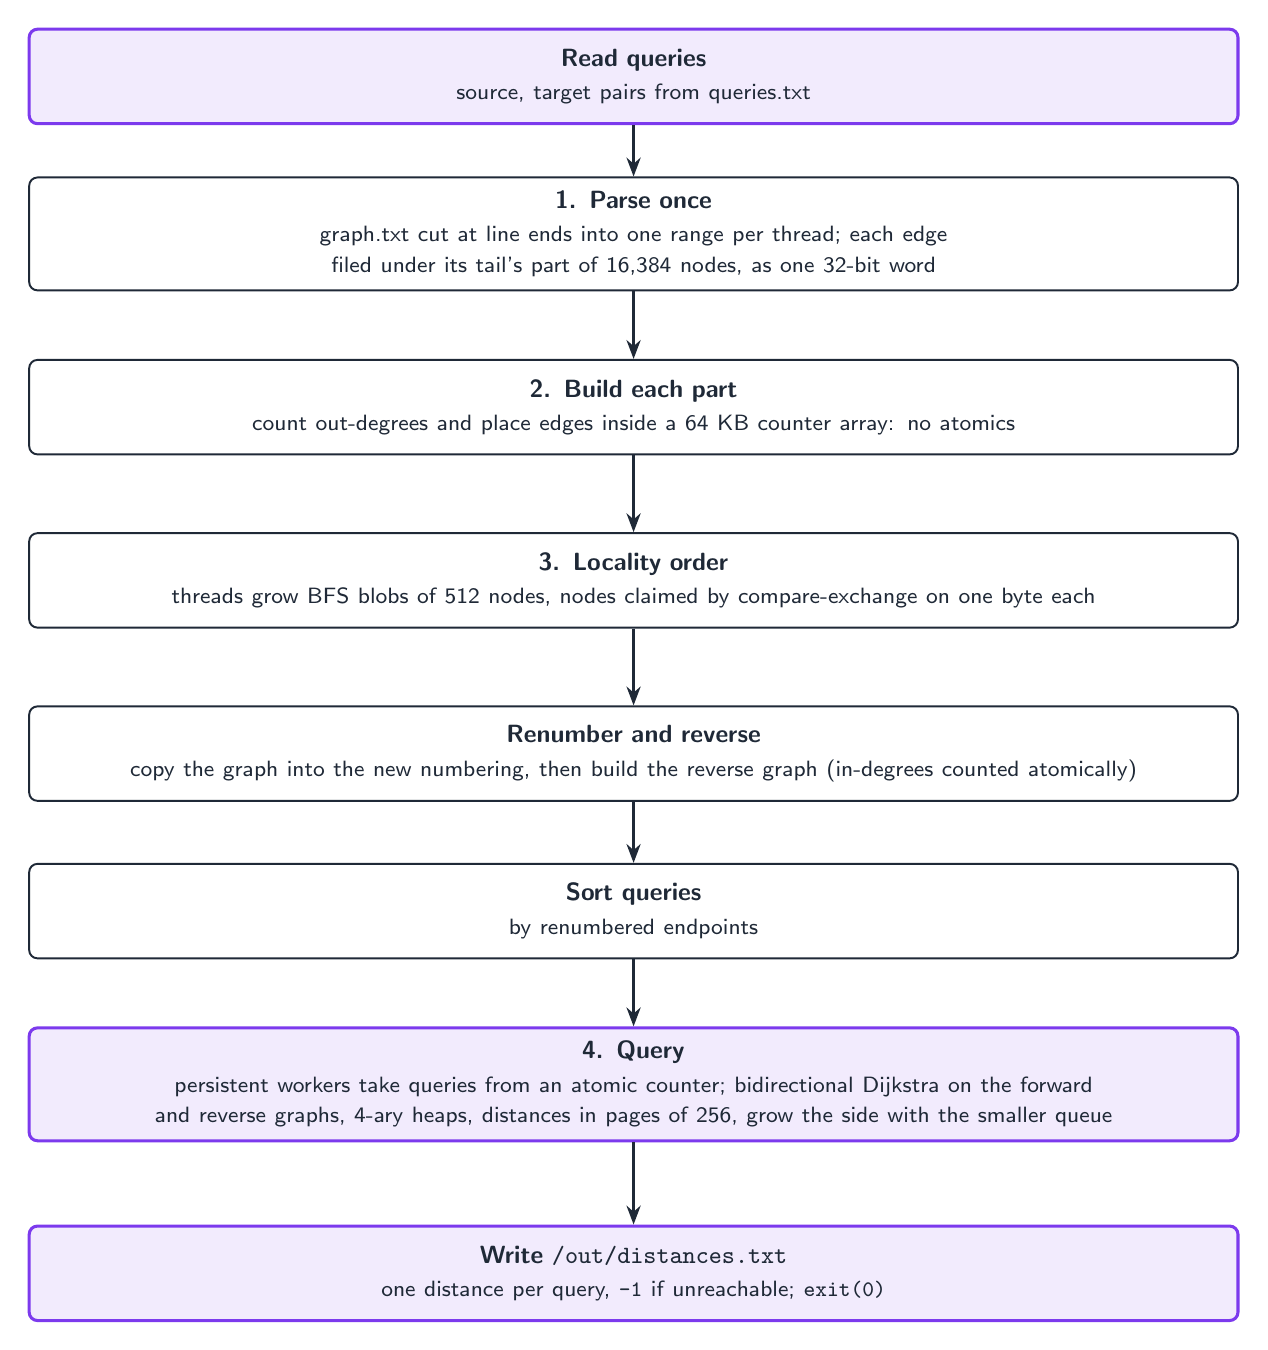
\begin{tikzpicture}
  \def\w{150mm}
  \node[box=\w, hl=cD] (q) at (0,0) {\nt{Read queries}{source, target pairs from queries.txt}};
  \node[box=\w] (p) at (0,-2.0) {\nt{1. Parse once}{graph.txt cut at line ends into one range per thread; each edge filed under its tail's part of 16,384 nodes, as one 32-bit word}};
  \node[box=\w] (b) at (0,-4.2) {\nt{2. Build each part}{count out-degrees and place edges inside a 64 KB counter array: no atomics}};
  \node[box=\w] (bf) at (0,-6.4) {\nt{3. Locality order}{threads grow BFS blobs of 512 nodes, nodes claimed by compare-exchange on one byte each}};
  \node[box=\w] (rn) at (0,-8.6) {\nt{Renumber and reverse}{copy the graph into the new numbering, then build the reverse graph (in-degrees counted atomically)}};
  \node[box=\w] (s) at (0,-10.6) {\nt{Sort queries}{by renumbered endpoints}};
  \node[box=\w, hl=cD] (dj) at (0,-12.8) {\nt{4. Query}{persistent workers take queries from an atomic counter; bidirectional Dijkstra on the forward and reverse graphs, 4-ary heaps, distances in pages of 256, grow the side with the smaller queue}};
  \node[box=\w, hl=cD] (o) at (0,-15.2) {\nt{Write \texttt{/out/distances.txt}}{one distance per query, \texttt{-1} if unreachable; \texttt{exit(0)}}};

  \draw[arr] (q) -- (p);
  \draw[arr] (p) -- (b);
  \draw[arr] (b) -- (bf);
  \draw[arr] (bf) -- (rn);
  \draw[arr] (rn) -- (s);
  \draw[arr] (s) -- (dj);
  \draw[arr] (dj) -- (o);
\end{tikzpicture}
\end{document}
